\documentclass[12pt]{article}
\usepackage[a4paper,left=1in,right=1in,top=1in,bottom=1in]{geometry}
\usepackage[utf8x]{inputenc}
\usepackage{gensymb}
\usepackage{indentfirst}
\usepackage{graphicx}
\graphicspath{{/home/dnehme/Dropbox/profissional/protocolos/ptc-validation-roms/ssh/figure/}}
\usepackage[abs]{overpic}
\usepackage{float}
\usepackage[brazil]{babel}
\usepackage{multirow}
\usepackage{lmodern}
\usepackage{titlesec}
\usepackage{xcolor}
\usepackage{natbib}

\setcounter{secnumdepth}{4}

\titleformat{\paragraph}
{\normalfont\normalsize\bfseries}{\theparagraph}{1em}{}
\titlespacing*{\paragraph}
{0pt}{3.25ex plus 1ex minus .2ex}{1.5ex plus .2ex}


\begin{document}

\begin{center}
	{\bf {\Large Protocolo de validação de simulações do ROMS}}
	\vspace{5mm}\par

	{\bf {\large Elevação da Superfície Livre do Mar}}
	\\
	\hrulefill
	\\
	
	{\bf Equipe:} {\it Douglas M. Nehme}\\
	\par
\end{center}

\tableofcontents

\newpage

\addcontentsline{toc}{section}{Apresentação}
\section*{Apresentação}
	\par Este protocolo descreve o processo de validação dos resultados de elevação da superfície livre do mar de simulações do ROMS usando dados de altimetria por satélite.
	
\section{Variáveis obtidas por satélite}
	\par Antes de descrever as variáveis possíveis de serem obtidas a partir das medidas feitas pelos altímetros é importante saber que a altitude em que um satélite se encontra é definida em relação ao elipsóide de referência e os altimetros medem a variação altimétrica, que é a distância de seu centro de massa à superfície da Terra, como representado na Figura \ref{fig:variaveis_altimetria}. Nesta figura, além do elipsóide de refrência, que é uma aproximação da crosta terrestre de forma esférica com seus pólos achatados, retrata-se o geóide, que é a superfície que o oceano assumiria na ausência de forças, como os ventos, correntes ou marés. O geóide terestre reflete o campo gravitacional do nosso planeta e é uma superfície equipotencial. Descata-se que o elipsóide e o geóide são superfícies coincidentes na linha do Equador.

	\begin{itemize}
		\item Elevação da Superfície Livre do Mar\footnote[1]{Dependendo da área da oceanografia a Elevação da Superfície Livre do Mar pode apresentar diferentes significados, sendo que o apresentado neste protocolo se refere ao aplicado na altimetria por satélite.} (\textit{Sea Surface Height} - SSH): Os altimetros medem a
		\item Elevação Média da Superfície Livre do Mar (\textit{Mean Sea Surface} - MSS): 
		\item Anomalia da Superfície Livre do Mar (\textit{Sea Level Anomlay} - SLA):
		\item 
	\end{itemize}

	\begin{figure}[h]
		\centering
		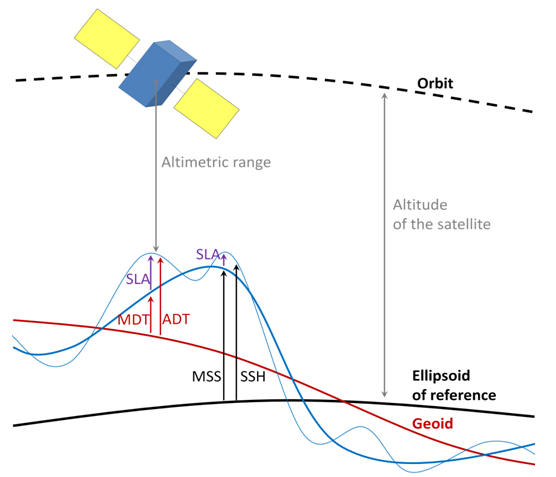
\includegraphics[width=\textwidth]{ABC_Altimetry.png}
   		\caption{BBB.
    	\label{fig:variaveis_altimetria}}
	\end{figure}

\section{Variável gerada pelo modelo}

\section{Comparação dos dados de satélite com os resultados do modelo}
	\par Além de descrever como é feita a comparação e quais variáveis são usadas, citar que o zeta do ROMS não é totalmente igual ao ADT por causa do efeito estérico da água, que é produzido por sua expansão térmica e não está presente em modelos que consideram a aproximação de Boussinesq.

\section{Produtos disponíveis}
	\par Falar dos prós e contras do produto Near Real Time e do Reprocessed que são a diferença entre tempo de latência e quantidade de dados utilizada.

\section{Download dos arquivos}
	
\bibliographystyle{coppe-plain}
\bibliography{biblio/biblio}
\addcontentsline{toc}{section}{Referências}

\end{document}
